\section{\texorpdfstring{\ZZ}{ZZ} Background}
\label{sec:bkg_ZZ}

While the \ZZ background is responsible for only 3\,\% of the background in the ten channels with highest overall sensitivity, its contribution is around 40\,\% in the 4-lepton regions.

The control region is defined by 4 leptons, 2 OSSF pairs (at least one on-\Z), and $\MET < 50\,\GeV$. We use \ZZ MC with fully leptonic decays and normalize the total number of events in the control region, after subtracting other backgrounds. The normalization factor is $1.38 \pm 0.23\stat$. Fig.~\ref{fig:ZZ} shows the 4$\ell$ mass distribution in the control region.

\begin{figure}
\begin{center}
	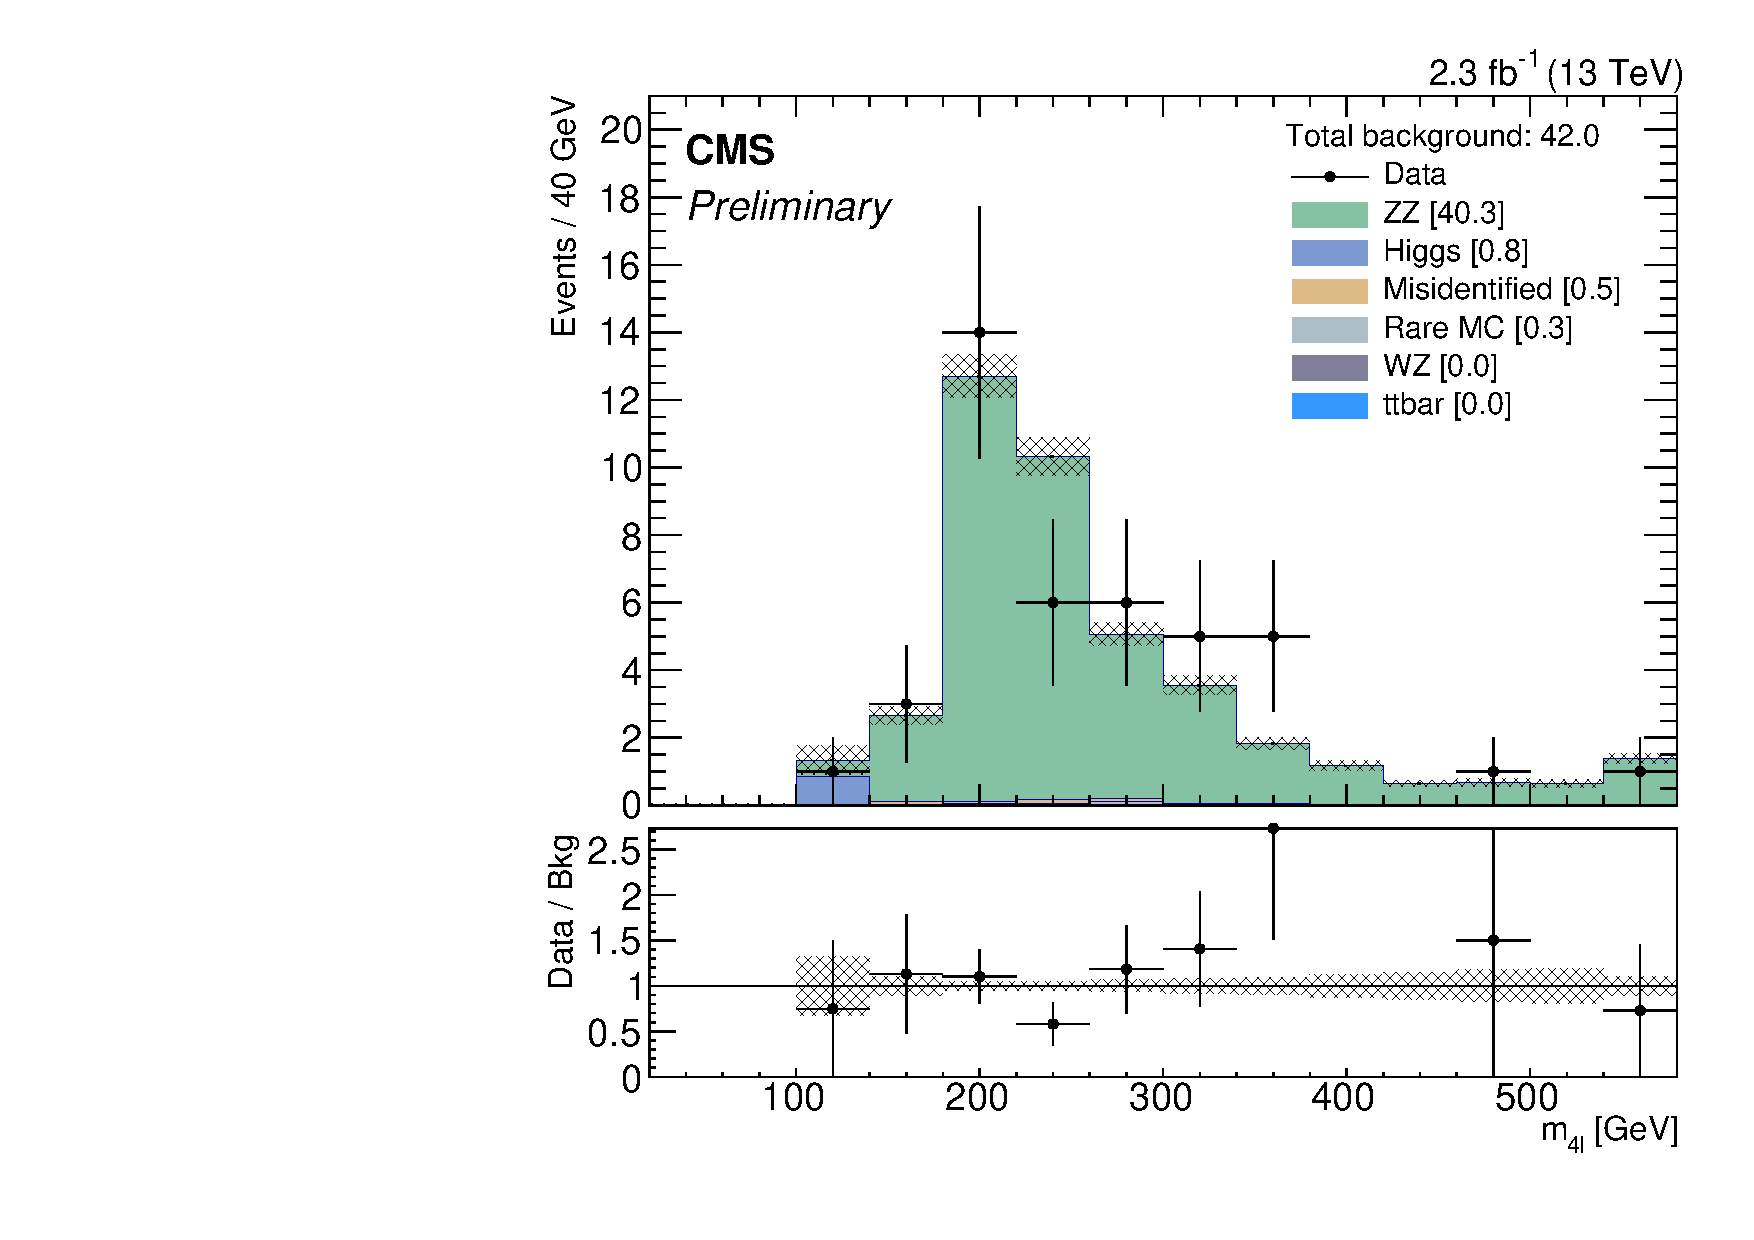
\includegraphics[width=.7\textwidth]{Background/bkg_ZZ/ZZ_DYz2MET0to50HT0to200_MLIGHTLEPTONS}
	\caption{The $m_{4\ell}$ distribution in the \ZZ control region. The last bin is the overflow. Uncertainty bands include both statistical and systematic uncertainties, with the exception of the \ZZ normalization uncertainty.
	\label{fig:ZZ}}
\end{center}
\end{figure}
